\section{Lektion 15-03-2018}

\begin{enumerate}
	\item Ørets opbygning
	\item Frekvensopfattelse
	\item Lydniveau
	\item Tonehøjde
	\item Lokalisering af lydkilder (retningsbestemmelse)
\end{enumerate}

\begin{mdframed}[style=exampledefault]
	\begin{itemize}
		\item \textbf{Pensum:} 
		\begin{enumerate}
			\item Master Handbook Of Acoustics, ch. 4
			\item Audio Meetering, sec. 7, 10
			\item Elektroakustik, TAS,  p. 7-11
		\end{enumerate}
		\item \textbf{Opgaver:} 
		\begin{enumerate}
			\item Lyd og Akustik - Lektion 3 - opgaver og øvelser
		\end{enumerate}
	\end{itemize}
\end{mdframed}

\subsection{Psykoakustik}
\begin{itemize}
	\item Transmissionen fra en lyd i den fysiske verden til en menneskelig opfattelse.
	\item Detektion via sanseapparatet (uden erkendelse) eller som et
	egentlig lydindtryk (med erkendelse).
\end{itemize}

\subsubsection{Psykometri}
\begin{itemize}
	\item Eksperiment med person under velkontrolerede forhold i en lydisoleret kabine. En uforstyrret forsøgsperson skal følge en simpel instruktion og afgive svar afhængigt af hvad	han eller hun hører. 
\end{itemize}

\subsection{Ørets opbygning}
\begin{itemize}
	\item Det ydre øre
	\begin{itemize}
		\item Består af et bruskskelet, beklædt med hud.
		\item Trommehinden, en membran, adskiller øregangen fra mellemøret.
	\end{itemize}
	\item Mellemøret
	\begin{itemize}
		\item Et luftfyldt hulrum mellem trommehinden og øresneglen.
		\item Er forbundet til svælget via en luftkanal, som sikrer at trykket i mellemøret kan udlignes med omgivelserne (flyve, dykke).
		\item Bygget op af 3 små knogler.
		\begin{itemize}
			\item Hammeren (malleus)
			\item Ambolten (incus)
			\item Stigbøjlen (stapes)
		\end{itemize}
		\item Øreknoglerne benytter vægtstangsprincippet til at overføre energien i vibrationerne fra trommehinden til væsken i det indre øre.
	\end{itemize}
\end{itemize}

\begin{figure} [H]
	\centering
	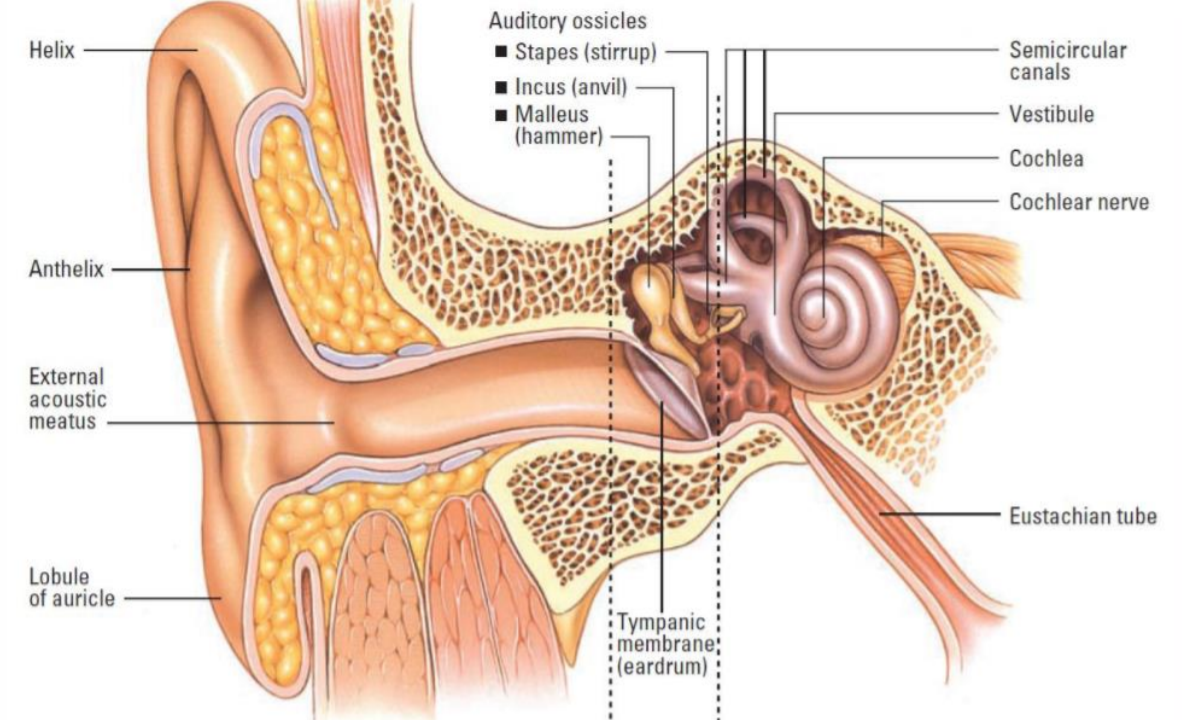
\includegraphics[width=\linewidth]{graphics/41.png}
	\caption{Ørets opbygning.}
	\label{fig:41}
\end{figure}

\begin{itemize}
	\item Det indre øre
	\begin{itemize}
		\item Består af øresneglen kaldet cochlea.
		\begin{itemize}
			\item Er ca 3.5 cm lang, Ø2mm og roterer ca 2.5 omgange.
			\item Indeholder sansetråde, der opfatter lydimpulser. 
			\item Lydbølgerne bliver omsat til elektriske nerveimpulser. 
		\end{itemize}
		\item Otoakustisk emission.
		\begin{itemize}
			\item Et normalt øre udsender selv lyde!
		\end{itemize}
	\end{itemize}
\end{itemize}

\subsection{Lydniveau}
\begin{itemize}
	\item Øret er ikke lige så sensitiv for bas toner ved lave lydniveauer.
	\item Inverteres kurverne fåes ørets frekvensrespons i forhold til lydniveau (vægtningskurver hvor A svarer til nedslidningen af hørelsen).
	\item 40-phon contour = \SI{40}{\decibel} lydtryksniveau ved \SI{1}{\kilo\hertz}.
	\item \Cref{fig:42} viser hvordan lydtryksniveaut ændres for forskellige frekvenser for at blive opfattet som samme lydstyrke som \SI{1}{\kilo\hertz} referencen ved 40 phon.
\end{itemize}

\begin{figure} [H]
	\centering
	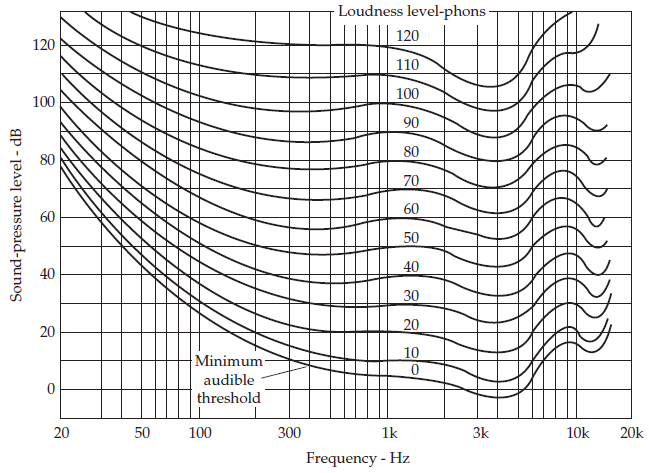
\includegraphics[width=\linewidth]{graphics/42.png}
	\caption{Equal-loudness contours of the human ear for pure tones.}
	\label{fig:42}
\end{figure}

\subsection{Frekvensopfattelse}
\begin{itemize}
	\item Frekvens er en objektiv parameter (generatorer, analysatorer).
	\item Pitch eller tonehøjde er en subjektiv parameter (pplevet).
	\begin{itemize}
		\item I midt-frekvens området er opfattelsen af	tonehøjde uafhænig af lydniveau.
		\item I lav- og højfrekvens området er opfattelsen af tonehøjde en lille smule lydniveau afhænig.
	\end{itemize}
\end{itemize}

\subsection{Tonehøjde}
\begin{itemize}
	\item Tonehøjden (pitch) af en frekvens høres forskelligt af øret.
	\item Tonehøjden for en \textbf{lav frekvens dæmpes} når intensiteten øges mens tonehøjden for en \textbf{høj frekvens øges} når intensiteten øges.
	\item Harmonisk er en lineær skala.
	\item Oktaver er en logaritmisk skala ofte anvendt i musik fordi den skalerer bedre til ørets opfattelse af lyd. 
	\begin{itemize}
		\item En oktav er defineret ved en 2:1 ratio af to frekvenser. 
		\item Intervallet fra \SI{100}{\hertz} til \SI{200}{\hertz} opfattes som værende større end intervallet fra \SI{200}{\hertz} til \SI{300}{\hertz}. 
	\end{itemize}
\end{itemize}

\begin{figure} [H]
	\centering
	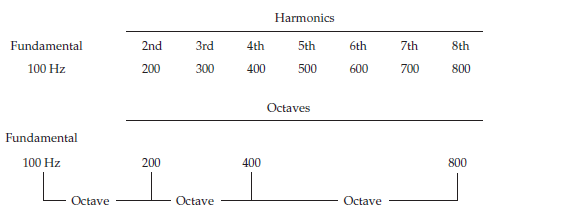
\includegraphics[width=\linewidth]{graphics/3.png}
	\caption{Sammenligning mellem harmoniske og oktaver. }
	\label{fig:3}
\end{figure}

\begin{equation}\label{eq:octave}
\frac{f_2}{f_1} = 2^n
\end{equation}

\begin{description}
	\item $f_2$ = frequency of the upper edge of the octave interval, \si{\hertz}
	\item $f_1$ = frequency of the lower edge of the octave interval, \si{\hertz}
	\item $n$ = number of octaves
\end{description}

\begin{itemize}
	\item Scopet af det hørbare spektrum er \SI{20}{\hertz} til \SI{20}{\kilo\hertz}.
	\begin{itemize}
		\item Der er lyde der ikke kan høres af øret. Det er frekvenser der er lavere end det hørbare spektrum (infrasound) og frekvenser der er højere end det hørbare spektrum (ultrasound).
	\end{itemize}
\end{itemize}

\subsection{Lokalisering af lydkilder}
\subsubsection{Retningsbestemmelse}
\begin{itemize}
	\item Øregangen fungerer som en kvart-bølge rør der er lukket i den ene ende af trommehinden og danner resonanser.
	\item Overførelsesfunktionen ved indgangen til øregangen ændres ved forskellige retninger (horisontal og vertikal) af lyden.
	\item Man kan retningsbestemme helt ned til \SI{1}{\degree} ændring i lydens lokation.
\end{itemize}
\subsubsection{Maskering}
\begin{itemize}
	\item En lyd kan overdøve (maskere) en anden lyd.
	\item \textbf{Simultan maskering} hvor det maskerende og det maskerede signal til stede samtidig.
	\begin{itemize}
		\item \textbf{Fuldstændig maskering} hvor det maskerede signal overdøves fuldstændigt af det maskerende signal. 
		\item \textbf{Partiel maskering} hvor det maskerede signal ikke overdøves fuldstændig, men den oplevede styrke (hørestyrken) påvirkes. 
		\item \textbf{Central maskering} hvor hørestyrken på det ene øre kan påvirkes af en lydpåvirkning af det andet øre.
	\end{itemize}
	\item \textbf{Pre-maskering} hvor et lydsignal maskeres af et efterfølgende kraftigere signal.
	\begin{itemize}
		\item Bagud i tid (ca. \SI{20}{\milli\second}).
		\item Ikke specielt afhængig af niveauet af det maskerende signal.
	\end{itemize}
	\newpage\item \textbf{Post-maskering} hvor et lydsignal maskeres af et forudgående kraftigere signal.
	\begin{itemize}
		\item Fremad i tid.
	 	\item Afhængig af maskeringssignalets varighed (kortere signal medfører kortere maskering). 
	\end{itemize}  
\end{itemize}
\begin{figure} [H]
	\centering
	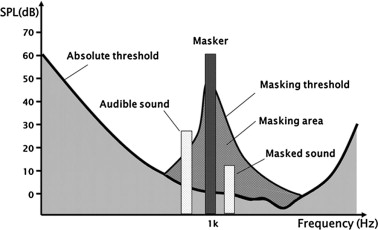
\includegraphics[width=.8\linewidth]{graphics/43.png}
	\caption{ \href{https://www.sciencedirect.com/science/article/pii/S0167639313000642}{Maskering.}}
	\label{fig:43}
\end{figure}